\section{Implementierung}
In diesem Kapitel geht es um die Implementierung und den Aufbau von Grafana, um \gls{Cyberangriff} mithilfe der \gls{mitre} Matrix zu erkennen. Das Labor wird mit einem \gls{container} und \glsfirst{vm} aufgebaut, wie im Diagramm in der Abbildung \ref{fig:Arbeitslabor} dargestellt.

\begin{figure}[H]
   \centering
   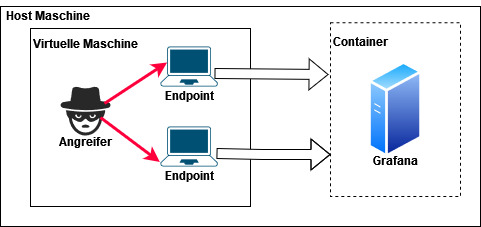
\includegraphics[width=1\textwidth]{assets/Arbeitslabor.jpg}
   \caption[Aufbau unseres Arbeitslabors]
   {Aufbau unseres Arbeitslabors \\Quelle: Eigene Quelle}
   \label{fig:Arbeitslabor}
   \centering
\end{figure}

Unser Aufbau verfolg folgende Ziele: die Aufnahme und Anpassung von Logdateien für Grafana, die Mustererkennung für ausgewählte \glsplural{Cyberangriff} und schließlich die Erstellung von Warnmeldungen für die Endnutzer, damit sie geeignete Sicherheitsmaßnahmen ergreifen können.

\newpage
Der gezielte Ablauf unserer Arbeit ist in der Abbildung \ref{fig:Ablauf_grafana2} dargestellt:

\begin{figure}[H]
   \centering
   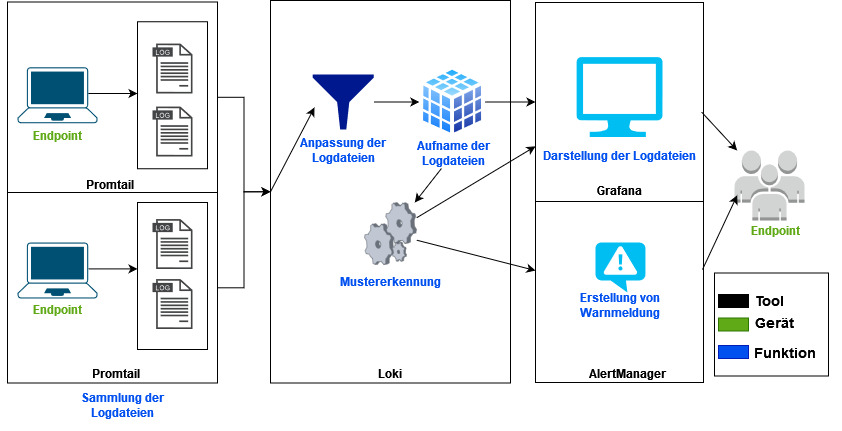
\includegraphics[width=1\textwidth]{assets/Ablauf_grafana2.jpg}
   \caption[Erwarteter Ablauf der Sammlung der Logdateien bis zur Warnmeldung]
   {Erwarteter Ablauf der Sammlung der Logdateien bis zur Warnmeldung \\ Quelle: Eigene Quelle und \citep{Grafana_loki}}
   \label{fig:Ablauf_grafana2}
   \centering
\end{figure}

\subsection{Angriffserkennung anhand der Mitre ATT\&CK Matrix}
Es gibt verschiedene Methoden und Frameworks, die von \gls{SOC}-Teams verwendet wird, um \glsplural{Cyberangriff} zu vermeiden, zu erkennen und zu unterbrechen.  Da sich die Richtlinien und Schwerpunkte dieser Frameworks und Methoden unterscheiden können und somit unterschiedliche Anforderungen an den Aufbau unserer Struktur stellen könnten, entschieden wir uns für die \gls{mitre} Matrix, insbesondere da dieses Framework auch in Splunk integriert ist.

Die \gls{mitre} Matrix hat folgenden Zwecke \citep{Mitre_Started}:

{\setstretch{1.5}
\begin{itemize}[noitemsep]
   \item Erkennung und Analyse von Angriffstechnik
   \item	strukturierte Datensammlung über Bedrohungen
   \item	Emulieren von \glsplural{Cyberangriff} für die Anwendung an Angriffsübungen
   \item	Systemhärtung und Verbesserung der Verteidigungsmaßnahmen
\end{itemize}
}

Die Matrix ermöglichen Unternehmen und \gls{SOC}-Teams umfassende Möglichkeiten, um ihre Ressourcen zu schützen und ihr Fachwissen im Bereich der \gls{Cybersicherheit} zu erweitern \citep{Hazel_howtousemitre}. In dieser Arbeit konzentrieren wir uns auf die Entwicklung und Implementierung einer Methode zur automatischen Erkennung und Analyse von Angriffstechniken in Grafana.

Die \gls{mitre} Matrix ist auf \glsfirst{ttp} basiert. Angriffe, Gegenmaßnahmen und Erkennung werden nach \gls{ttp} definiert. Die Matrix besteht aus 14 Taktiken, zu denen jeweils Techniken gehören, die wiederum in Sub-Techniken unterteilt sind. Jede Sub-Technik wird mit Beispielen, Härtungsmaßnahmen und Erkennungsregeln beschrieben. Die nächste Abbildung, \ref{fig:ttp}, zeigt, wie die \gls{ttp} aufgebaut werden:

\begin{figure}[H]
   \centering
   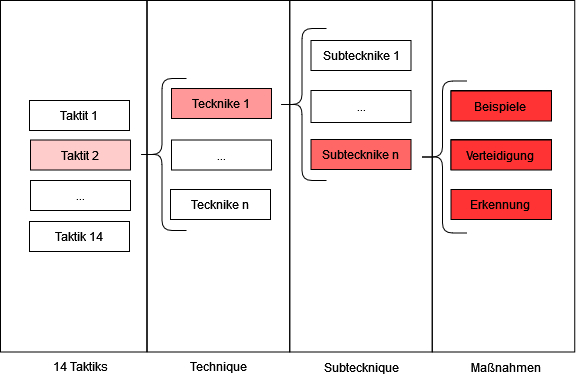
\includegraphics[width=0.8\textwidth]{assets/Mitre_structure.drawio.png}
   \caption[Struktur der \gls{mitre} Matrix]
   {Struktur der \gls{mitre} Matrix \\Quelle: Eigene Quelle und \citep{Mitre_Started}}
   \label{fig:ttp}
   \centering
\end{figure}

% {\setstretch{1}
% Die 14 Taktiks sind folgende:
% \begin{itemize}[noitemsep]
%    \item Informationssammlung für zukünftige Angriffe
%    \item	Entwicklung von Ressource von Angreifer
%    \item Erster Zugang zum Opfersysteme
%    \item Ausführung von bösartigen Coden
%    \item Beharrlichkeit von System
%    \item	Privilegienausweitung
%    \item Vermeidung von Verteidigungssysteme
%    \item \textbf{Zugang zu Anmeldedaten}
%    \item Umgebungserkennung
%    \item Seitliche Bewegung zu anderem Systemen innerhalb des Angriffsziels
%    \item interne Informationssammlung
%    \item Steuerung und Kontrolle (C2 - Command and Control im Original)
%    \item Datenextrahierung
%    \item	Auswirkung auf die Integrität
% \end{itemize}
% }

\newpage
\subsection{Auswahl des Angriffes}
In dieser Arbeit beschäftigen wir uns mit der Taktik \quotes{Zugang zu Anmeldedaten} und deren Technik \gls{bruteforce}. Diese Technik ist in vier Untertechniken aufteilt:

In dieser Arbeit beschäftigen wir uns mit der Taktik \quotes{Zugang zu Anmeldedaten} und ihrer Technik \quotes{\gls{bruteforce}}. Diese Technik ist in vier Untertechniken unterteilt:

{\setstretch{1}
\begin{itemize}[noitemsep]
   \item \gls{bruteforce}
   \item	Entschlüsselung von \glsplural{hash}
   \item \textit{\gls{stuffing}}
   \item \textit{\gls{spraying}}
\end{itemize}
}

Da unser Ziel hier ist, Grafana zu verwenden, um Angriffe zu erkennen, haben wir uns für einen einfachen und reproduzierbaren Angriff entschieden, der wenige Ressourcen erfordert. In diesem Fall kann ein \gls{bruteforce} mit zwei \glsplural{vm} problemlos durchgeführt werden. Für diesen Angriff verwenden wir die Sub-Technik "Erraten von Anmeldedaten und \textit{\gls{stuffing}}, da sie ähnliche Erkennungsmethoden aufweisen. Da unser Fokus bei dieser wissenschaftlichen Arbeit auf der Angriffserkennung schließen andere Maßnahmen  wir hierbei aus.

Die nächste Abbildung, \ref{fig:Unser_ttp}, zeigt den Umfang unseres Implementationsversuchs mithifel von \gls{mitre}:
\begin{figure}[H]
   \centering
   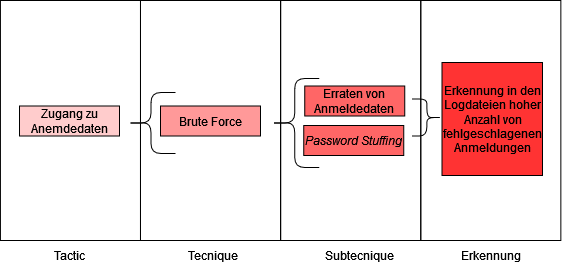
\includegraphics[width=0.7\textwidth]{assets/T1110.drawio.png}
   \caption[\glsfirst{ttp} für unseren Angriff]
   {\glsfirst{ttp} für unseren Angriff \\Quelle: Eigene Quelle und \citep{Mitre_t1110}}
   \label{fig:Unser_ttp}
   \centering
\end{figure}

\newpage
\subsection{Installation und Generierung von Logdateien}
In diesem Abschnitt konzentrieren wir uns auf die folgenden Punkte:

\begin{enumerate}[noitemsep]
   \item Einrichtung von \glsplural{vm} für das Opfersystem und den Angreifer
   \item Simulation des Angriffe zur Erzeugung von Logdateien
   \item Installation und Konfiguration von Grafana Loki und Promtail mit \gls{container}
   \item Weiterleitung der Logdateien an Grafana
\end{enumerate}

Die Installation und Verwendung können entweder über eine \glsfirst{GUI} des Betriebssystems oder über die Kommandozeile durchgeführt werden. In dieser Arbeit verwenden wir die Kommandozeile.

\subsubsection{Einrichtung der \glsplural{vm} für Opfersystem und Angreifen}
Die beiden \glsplural{vm} sind eine \quotes{\gls{kali} \glsfirst{vm}} und \quotes{\gls{ubuntu} Server 22.04.2} mit standardmäßigen Einstellungen. Beide Maschinen wurden entsprechend ihrer jeweiligen Dokumentation installiert \citep{kali_vm} und \citep{Ubuntu_server}.

Für das Opfersystem haben wir uns für die Passwörter \quotes{qwertz} und \quotes{password} entschieden. Laut einer Umfrage gehören diese Passwörter zu den zehn am häufigsten verwendeten Passwörtern in Deutschland \citep{silicon_passwort}. Für die Durchführung des \gls{spraying} haben wir folgende Benutzername-Passwort Kombinationen erstellt:

{\setstretch{1.0}
\begin{lstlisting}[frame=single]
            Opfersystem 1          Opfersystem 2
            admin:123456           bob:hallo
            user1:passwort         master:alice
            user2:abc123           hans:daniel
            user3:qwertyuiop       bruno:super123
\end{lstlisting}
}

\newpage
\subsubsection{Generierung von Logdateien mit der Angrifsssimulation}
Für den Angriff verwenden wir folgende Tools:

{\setstretch{1.0}
\begin{itemize}[noitemsep]
   \item	\glsfirst{ssh}
   \item \gls{hydra}
\end{itemize}
}

In diesem Szenario sendet \gls{hydra} gleichzeitig mehrere Authentifizierungsversuche an das Opfersystem, um eine \gls{ssh}-Verbindung herzustellen. Das Tool verwendet ein sogenanntes Wörterbuch mit verschiedenen Einträgen, die als Passwörter dienen. Für unseren Test benutzen wir die bekannte \gls{rockyou}-Wörterbuch.

Die Abbildung \ref{fig:stuffing} zeigt, wie das \gls{stuffing} abläuft:
\begin{figure}[H]
   \centering
   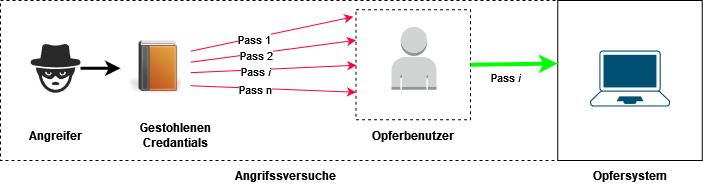
\includegraphics[width=1\textwidth]{assets/Stuffing.png}
   \caption[Darstellung von \textit{\gls{stuffing}}]
   {Darstellung von \textit{\gls{stuffing}} nach \cite{Nguyen_stuffing}}
   \label{fig:stuffing}
   \centering
\end{figure}

In diesem Angriff versucht der Angreifer sich mit einem Konto anzumelden, indem er mit vielen Passwörter aus dem Wörterbuch probiert, bis eins richtige gefunden ist. Es können mehrere Anmeldungsversuche geschickt werden, bis eine von denen funktioniert.

\newpage
\gls{stuffing} wurde mit folgendem Kommando durchgeführt \citep{kali_hydra}:
%Verbatim
{\setstretch{1.0}
\begin{Verbatim}[frame=single]
hydra -l [Benutzername] -P rockyou.txt [Opfersystem] ssh -V -t 4

# Erklärung
-l: Spezifikation des Benutzernamens, den wir angreifen
-P: Auswahl der Datei mit bekannten Passwörtern
ssh: Auswahl der Anwendung, die wir angreifen
-V: Ausführliche Ausgabe über Versuche, Fehler und Erfolg
-t 4: Anzahl von gleichzeitigen Verbindungen
\end{Verbatim}
}

Die Abbildungen \ref{fig:Ausgabe_Stuffing_Opfer1} und \ref{fig:Ausgabe_Stuffing_Opfer2} zeigen ein Teil der Ausgabe von \gls{hydra} während der Ausführung von \gls{stuffing} gegen das Opfersystem1 und Opfersystem2:
\begin{figure}[H]
   \centering
   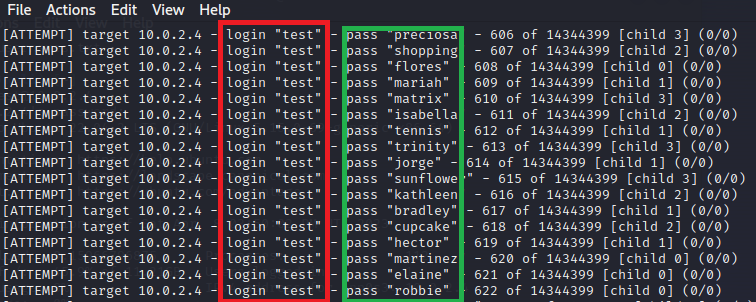
\includegraphics[width=0.9\textwidth]{assets/stuffing_kali.png}
   \caption[Ausgabe von \textit{\gls{stuffing}} gegen Opfersystem1]
   {Ausgabe von \textit{\gls{stuffing}} gegen Opfersystem1}
   \label{fig:Ausgabe_Stuffing_Opfer1}
   \centering
\end{figure}

\begin{figure}[H]
   \centering
   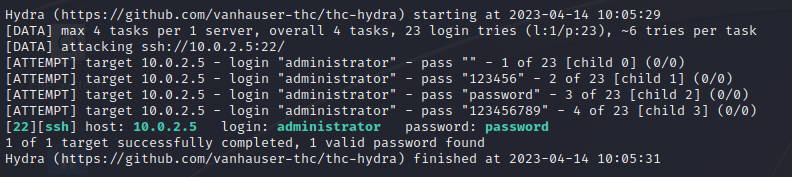
\includegraphics[width=1\textwidth]{assets/stuffing_kali2.png}
   \caption[Ausgabe von \textit{\gls{stuffing}} gegen Opfersystem2]
   {Ausgabe von \textit{\gls{stuffing}} gegen Opfersystem2}
   \label{fig:Ausgabe_Stuffing_Opfer2}
   \centering
\end{figure}

Auf den Abbildungen \ref{fig:Ausgabe_Stuffing_Opfer1} und \ref{fig:Ausgabe_Stuffing_Opfer2} sehen wir in rot markiert, dass der Angriff den Benutzernamen \quotes{test} im Opfersystem1 und \quotes{Administrator} Opfersystem2 zielt. In grün werden die verschiedenen Passwörter aus \gls{rockyou}-Wörterbuch verwendet. Auf der Abbildung \ref{fig:Ausgabe_Stuffing_Opfer2} wird das gefundene Passwört grün geschrieben.

Unser nächster Angriff, \gls{spraying}, ist in der Abbildung \ref{fig:spraying} dargestellt:
\begin{figure}[H]
   \centering
   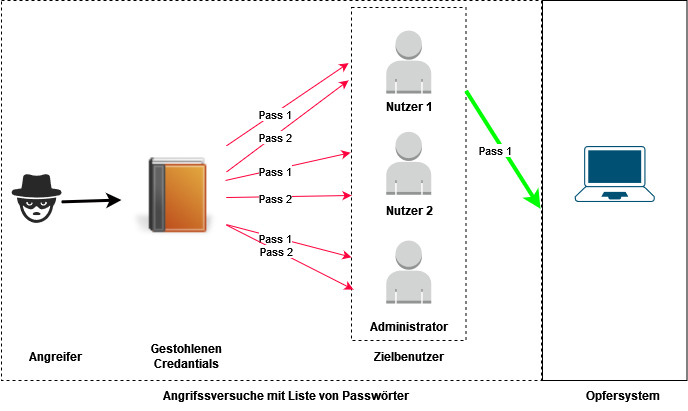
\includegraphics[width=0.9\textwidth]{assets/Spraying.jpg}
   \caption[Darstellung von \textit{\gls{spraying}}]
   {Darstellung von \textit{\gls{spraying}}\\Quelle: Eigene Quelle und \citep{Swathi_spraxy}}
   \label{fig:spraying}
   \centering
\end{figure}

Aus der Abbildung \ref{fig:spraying} sehen wir, dass bei \gls{spraying} weniger Passwörter im Vergleich zum \gls{stuffing} verwendet werden. In diesem Fall werden gegen mögliche viele existierenden Benutzername versucht. Hier will der Angreifer  Kontosperrungen vermeiden und gegenüber Sicherheitsmaßnamen Unauffälig bleiben.

Für diesen Angriff benutzen wir folgendes Kommando:
{\setstretch{1.0}
\begin{Verbatim}[frame=single]
hydra -L username2.txt -P passwoerter.txt [Opfersystem2] ssh -V -t 4
-L: Auswahl der Datei mit gefunden Benutzernamen
\end{Verbatim}
}

In diesem Fall gehen wir davon aus, dass der Angreifer einige oder alle Benutzernamen bereits kennt. Da bei diesem Angriff weniger Anmeldeversuche pro Nutzer durchgeführt werden, verwenden wir eine selbst erstellte Datei mit weniger Passwörtern als die \gls{rockyou}-Datei. Unsere Datei enthält die am häufigsten verwendeten Passwörter in Deutschland \citep{silicon_passwort}.

Die Abbildungen \ref{fig:spraying_opfer1} und \ref{fig:spraying_opfer2} zeigen die Ausgabe von \gls{spraying}:
\begin{figure}[H]
   \centering
   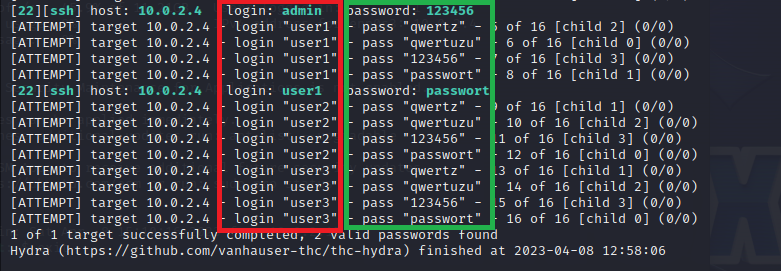
\includegraphics[width=1\textwidth]{assets/Spraying_Kali.png}
   \caption[Ausgabe von \textit{\gls{spraying}} in Kali Linux gegen Opfersystem1]
   {Ausgabe von \textit{\gls{spraying}} in Kali Linux gegen Opfersystem1}
   \label{fig:spraying_opfer1}
   \centering
\end{figure}

\begin{figure}[H]
   \centering
   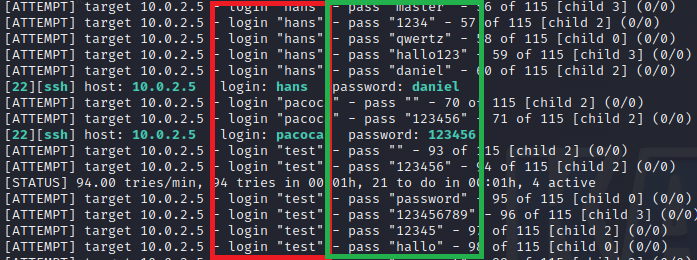
\includegraphics[width=1\textwidth]{assets/Spraying_Kali2.png}
   \caption[Ausgabe von \textit{\gls{spraying}} in Kali Linux gegen Opfersystem2]
   {Ausgabe von \textit{\gls{spraying}} in Kali Linux gegen Opfersystem2}
   \label{fig:spraying_opfer2}
   \centering
\end{figure}

Die Abbildungen \ref{fig:spraying_opfer1} und \ref{fig:spraying_opfer2} zeigen die verschiedenen Benutzername (rot markiert) aber wenige Passwörter pro Nutzer (grün markiert). Auf beiden Abbildungen werden die gefundenen Passwört grün geschrieben.

Nach den Durchführungen dieser Simulationen generierten wir drei Logdateien mit insgesamt 40 KB Größe.

\newpage
\subsubsection{Installation und Einrichtung von Grafana, Loki und Promtail}
Für die Einrichtung haben wir sowohl offizielle Dokumentation von Grafana als auch auf externe Quellen zurückgegriffen, um die Einstellungen an unsere Umgebung anzupassen \citep{Polinowski_PGL}. In den Anhänge \ref{appendix:orgGrafana} und \ref{appendix:AngepasstGrafana} befinden sich die heruntergeladenen originalen Konfigurationsdatei und die an unsere Umgebung angepasst. Diese Dateien benutzten wir für die Installation, Einstellung und Verwendung der Applikationen in \glsplural{container}.

% Unten befinden sich die von Grafana zur Verfügung gestellten Konfigurationsdateien und Installationsverfahren \citep{GrafanaLoki_run}:

% {\setstretch{1.0}
% \begin{lstlisting}[frame=single]
% wget https://raw.githubusercontent.com/grafana/loki/v2.8.0/cmd/
% loki/loki-local-config.yaml -O loki-config.yaml
% (die Datei wurde angepasst)

% wget https://raw.githubusercontent.com/grafana/loki/v2.8.0/
% clients/cmd/promtail/promtail-docker-config.yaml
% -O promtail-config.yaml (die Datei wurde angepasst)

% docker-compose -f docker-compose.yaml up
% \end{lstlisting}
% }

% \begin{enumerate}[noitemsep]
%    \item Herunterladen der Konfigurationsdatei von Loki
%    \item Herunterladen der Konfigurationsdatei von Promptail
%    \item Ausführung von dem \glsplural{container}, indem beide Konfigurationsdateien in eine eingepackt und angepasst wurden und schließlich von der \gls{container}-Anwendung gelesen werden
% \end{enumerate}

%Für spezifische Versionen oder weitere Einstellungen bietet die Dokumentation umfangreiche Möglichkeiten an \citep{GrafanaLoki_run}.

Für diesen ersten Test wurden die Logdateien des Opfersystems manuell auf den \gls{container} übertragen, da wir hier nur eine Instanz von Promtail verwendeten.  Für unsere Arbeit nahmen wir die folgenden Versionen von den Anwendungen:

\begin{table}[h]
   \centering
   \setstretch{1.2}
   \begin{tabular}{|c|c|}
   \hline
   \textbf{Anwendung}  & \textbf{Angewandte Version}  \\ \hline
   Grafana             & \cellcolor{green!25}9.5.2    \\ \hline
   Loki                & \cellcolor{green!25}2.8.2    \\ \hline
   Promtail            & \cellcolor{green!25}2.8.2    \\ \hline
   \end{tabular}
   \caption[Verwendete Versionen der Anwendungen]
   {Verwendete Versionen der Anwendungen \\Quelle: \citep{Grafana_Version} und \citep{GrafanaLoki_Version}}
   \label{tab:Versions}
\end{table}

% Die Entscheidung, eine ältere Version für Loki zu wählen, basierte auf Recherchen im offiziellen Forum von Grafana Loki. Viele Nutzer berichteten von Problemen mit ihren Abfragen. In verschiedenen Kommentaren wurde vorgeschlagen, einige Werte in der Konfigurationsdatei von Loki anzupassen, um die Leistung der Anwendung zu verbessern. Diese Lösungen waren für die meisten Forenteilnehmer jedoch erfolglos. Die Mehrheit der Teilnehmer gab außerdem an, dass Versionen über 2.4.1 dasselbe Problem aufweisen, weshalb sie die Version 2.4.1 verwendet haben \citep{githubforum}.

\newpage
\newgeometry{right=30mm, left=30mm}
\thispagestyle{lscape}
\begin{landscape}
   Nach der Ausführung des Kommandos ist die Anwendung benutzbar, wie in der Abbildung \ref{fig:grafana_welcome} dargestellt:
    \begin{figure}[H]
       % \centering
        \centerline{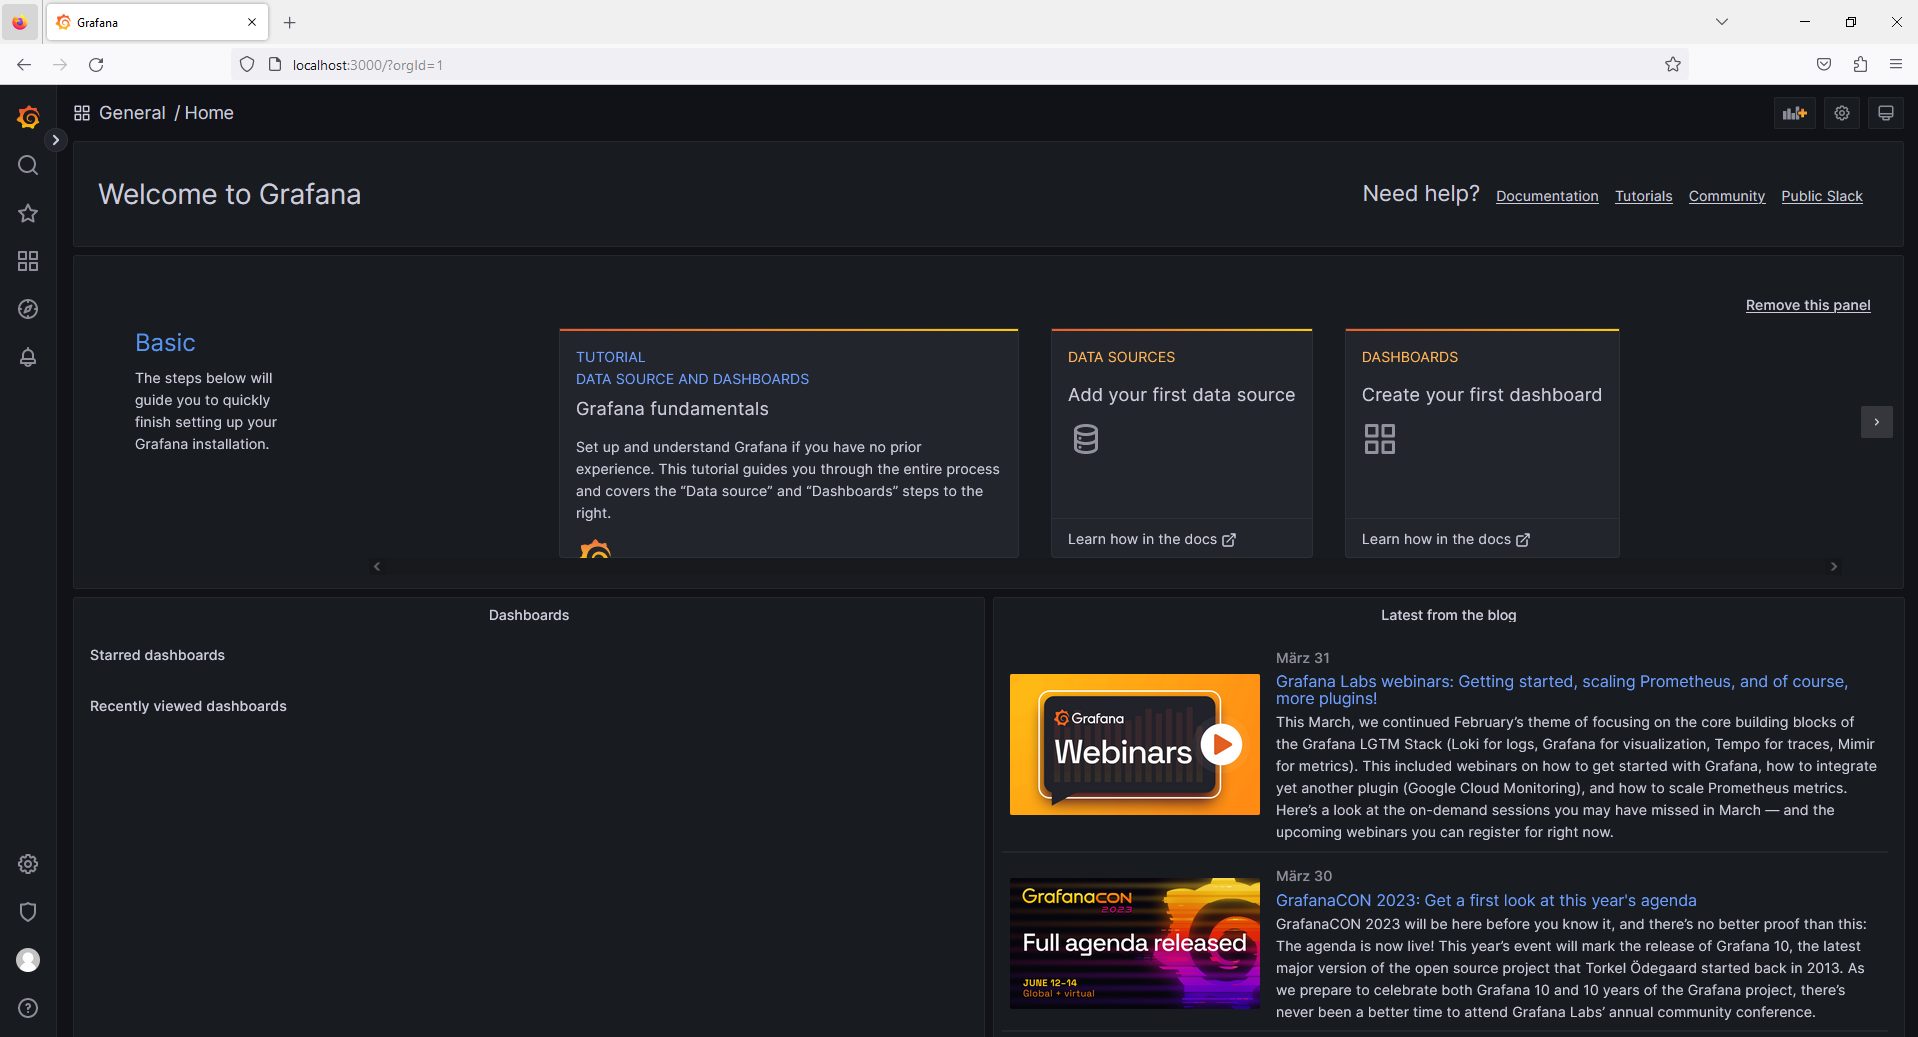
\includegraphics[width=1.5\textwidth]{assets/Installation_Grafana.png}}
        %\includegraphics[width=1.2\textwidth]{assets/5.4.2_1_Abb.jpeg}
        \caption[Screenshot der Willkommensseite von Grafana Loki]
        {Screenshot der Willkommensseite von Grafana Loki\\Quelle: Eigene Quelle und \citep{Grafana_Logs}}
        \label{fig:grafana_welcome}
        \centering
    \end{figure}
\end{landscape}
\restoregeometry

\subsubsection{Weiterleitung der Logdateien zu Grafana}
Grafana Loki bietet interne und externe Möglichkeiten Logdateien zu empfangen. Die internen beziehen sich auf Grafana Tools, während die externen unabhängige Methode von Grafana benutzen:

\begin{enumerate}[noitemsep]
   \item \textbf{interne Methode}:
   \begin{enumerate}[noitemsep]
      \item Promtail
      \item Grafana Agents
   \end{enumerate}
   \item \textbf{externe Methode}
   \begin{enumerate}[noitemsep]
      \item \glsfirst{API}
      \item \gls{opentelemetry}
   \end{enumerate}
\end{enumerate}

In unserer Arbeit verwenden wir \textbf{Promtail}, der in einem \gls{container} läuft. Diese Instanz sendet die von uns ausgewählten Logdateien an Grafana und verarbeitet alle Dateien innerhalb eines sogenannten \quotes{jobs}. Promtail kann Logdatein nur zu Grafana Loki oder zu anderen Promtail-Instanz schicken \citep{Grafana_Promtail}. Die Abbildung \ref{fig:Integration_Loki_Promtail_Grafana} auf der Seite \pageref{fig:Integration_Loki_Promtail_Grafana} zeigt diese beschriebene Struktur.

In einer produktiven Umgebung ist die Installation von \textbf{Grafana Agents} auf jedem \gls{Endpoint} eine andere Lösung, um Grafana Loki mit Logdateien zu füllen. Während Promtail Logdatei nur zu Loki schickt, kann Grafana Agents Logdateien zu \gls{prometheus}, OpenTelemetry und zu Tools von \textit{\gls{GrafanaSystem}}, wie \gls{mimir}, \gls{tempo}, \gls{phlare}, Loki und Grafana \citep{Grafana_Agents}.

\newpage
Die nächste Abbildung, \ref{fig:GrafAgents}, zeigt den Kommunikationfluss zwischen Grafana Agents und die integrieten Tools:

\begin{figure}[H]
   \centering
   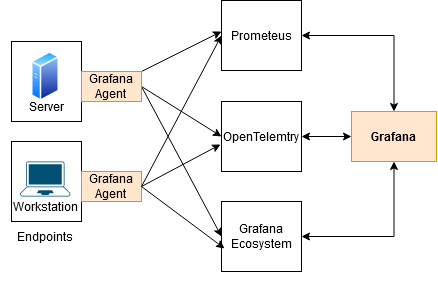
\includegraphics[width=0.7\textwidth]{assets/GrafanaAgents.drawio.png}
   \caption[Kommunikation zwischen Grafana Agents, \gls{prometheus}, OpenTelemetry und \textit{\gls{GrafanaSystem}}]
   {Kommunikation zwischen Grafana Agents, \gls{prometheus}, OpenTelemetry und \textit{\gls{GrafanaSystem}}\\Quelle: \citep{Grafana_Agents}}
   \label{fig:GrafAgents}
   \centering
\end{figure}

Der Kommunikationsfluss bei Grafana Agents funktioniert ähnlich, wie bei Promtail. Die \glsplural{Endpoint} (links), wo die Agents installiert sind, schicken die Logdateien zu den kompatiblen Tools (mitte), die sich wiederum mit Grafana (rechts) kommunizieren.

Die Sendung des Inhalts der Logdateien findet auch mithilfe von Grafana Loki \gls{http} \textbf{\gls{API}} statt. In diesem Fall werden die Zeile der Logdateien und nicht der Datei zum \gls{Endpoint} von Loki mit \gls{http} POST-Anfrage geschickt.

Grafana Loki bietet auch eine Integration mit dem Open-Source-Tool \gls{opentelemetry} an, um Logdateien zu empfangen \citep{Grafana_opentelemetry}. Die Integration mit Grafana Loki erfolgt über die Nutzung von \glsplural{API}. Der \textit{Collector} läuft in derselben Umgebung wie Grafana Loki, damit er die Logdateien empfangen und verarbeiten kann. Die \textit{Agents} laufen auf jedem Endpunkt und kommunizieren mit dem \textit{Collector}.

\newpage
Die folgende Abbildung stellt das Kommunikationsverfahren zwischen \gls{opentelemetry} und die Tools von \textit{\gls{GrafanaSystem}}:

\begin{figure}[H]
   \centering
   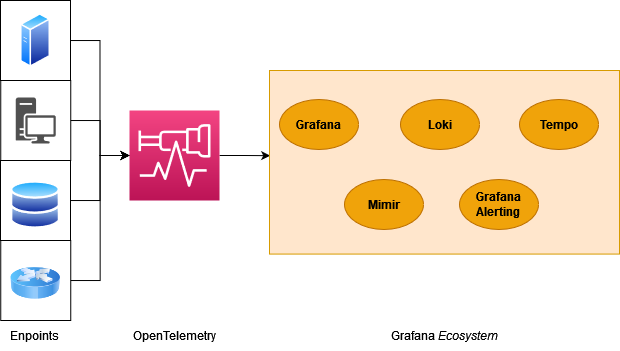
\includegraphics[width=0.8\textwidth]{assets/OpenTelemtry.png}
   \caption[Datenfluss zwischen \gls{opentelemetry} und die Tools von \textit{\gls{GrafanaSystem}}]
   {Datenfluss zwischen \gls{opentelemetry} und \textit{\gls{GrafanaSystem}}\\Quelle: \citep{Grafana_WhatOpentelemetry}}
   \label{fig:UsingOpenTelemetry}
   \centering
\end{figure}


Auf der linken Seite der Abbildung \ref{fig:UsingOpenTelemetry} haben wir die verschiedenen \glsplural{Endpoint}, auf denen jeweils ein \textit{Collector} läuft. In der Mitte ist der OpenTelemetry \glsplural{Endpoint}, der die Datei sammelt und dessen Inhalt verarbeitet. Diese werden schließlich an die Tools von \textit{\gls{GrafanaSystem}} weiterleitet.

\newpage
\subsection{Aufbau der Erkennungsregel für den ausgewählten Angriff}
Ein \gls{bruteforce} lässt sich durch eine hohe Anzahl der fehlgeschlagenen Anmeldeversuche erkennen \citep{Selvaganesh_SplunkBruteForce}. Wir betrachten eine Situation, in der keine Gegenmaßnahmen wie Kontosperre nach \textit{n} beliebigen Versuchen oder \gls{mfa}, implementiert sind. Das folgende Abbildung, \ref{fig:Aktivitaetsdiagramm_Anmeldung}, stellt Diagramm mit einem allgemeinen Ablauf eines Anmeldungsverfahrens dar:

\begin{figure}[H]
   \centering
   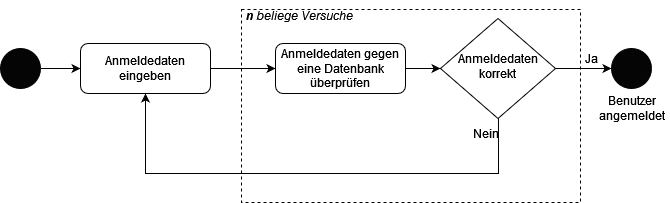
\includegraphics[width=0.8\textwidth]{assets/Anmeldeverfahren.drawio.png}
   \caption[Allgemeiner Ablauf eines Anmeldungsverfahrens]
   {Allgemeiner Ablauf eines Anmeldungsverfahrens \\Quelle: Eigene Quelle und \citep{Selvaganesh_SplunkBruteForce}}
   \label{fig:Aktivitaetsdiagramm_Anmeldung}
   \centering
\end{figure}

Grafana bietet ein Konfigurationsmuster für die Eingabe und Darstellung von \gls{ssh} Eventds an. In dieser Konfiguration sind bereits Regesätze für die
Verarbeirtung der Log-Einträge in Loki und Quellcode für die Generierung von Grafik in Grafana. Diese Konfigurationsdatei ermöglicht eine umfassende Analyse dieser Daten \citep{VoidQuark_sshlogs}. Die gesentet Logdateien werden mithilfe der folgenden Elemente gelesen und verarbeitet:

% % \begin{table}[H]
% %    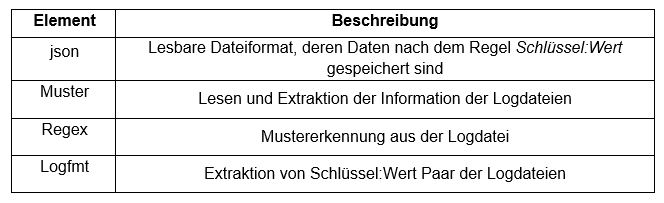
\includegraphics[width=\linewidth]{assets/tabelle_sshgrafana.png}
% %    \caption[Elementen eines Regelsätzes in Grafana Loki]
% %    {Elementen eines Regelsätzes in Grafana Loki \\Quelle: Eigene Quelle, \citep{VoidQuark_sshlogs} und \citep{Setter_Logfmt}}
% % \end{table}


\begin{table}[H]
   \setstretch{1.2}
   \begin{tabularx}{\textwidth}{|c|X|}
   \hline
   \multicolumn{1}{|c|}{\textbf{Element}} & \multicolumn{1}{|c|}{\textbf{Beschreibung}} \\
   \hline
      \glsfirst{json} & Lesbare Dateiformat, deren Daten nach dem Regel Schlüssel-Wert-Paar  gespeichert sind \\
   \hline
      Muster & Lesen und Extraktion der Information der Logdateien \\
   \hline
      \glsfirst{RegExp} & Mustererkennung aus der Logdatei \\
   \hline
      Logfmt & Extraktion von Schlüssel:Wert Paar der Logdateien \\
   \hline
   \end{tabularx}
   \caption[Elementen eines Regelsätzes in Grafana Loki]
   {Elementen eines Regelsätzes in Grafana Loki \\Quelle: Eigene Quelle, \citep{VoidQuark_sshlogs} und \citep{Setter_Logfmt}}
\end{table}


%https://grafana.com/docs/loki/latest/fundamentals/labels/
%https://prometheus.io/docs/concepts/jobs_instances/

Für jedes Angriffszenario benutzen wir spezifische Regeln, die mit \gls{logql} aufgebaut sind. Die Filterung findet mithilfe von zweil Labels \quotes{instance} und \quotes{job} statt. In Promtail wird jeder \gls{Endpoint} als \quotes{Instance} bezeichnet. Eine oder mehrere \quotes{instances} werden einem \quotes{job} zugewiesen. \quotes{jobs} beziehen sich auf die Bearbeitung der Logdateien nach dem spezifizieren Regeln, in unserem Fall, Überprüfung von \gls{ssh}-Logdateien. Diese Struktur stammt aus dem Tool \gls{prometheus}. Alle unsere \quotes{instance} werden in einem \quotes{job} eingepackt, wo sie nach den gleichen Regeln verarbeitet. Zusätliche Labels können auch definiert werde \citep{Prometheus_JobInstance}. Das folgende Diagramm, \ref{fig:Labels_GrafanaLoki}, stellt die Beziehung zwischen dieser beiden Labels dar:

\begin{figure}[H]
   \centering
   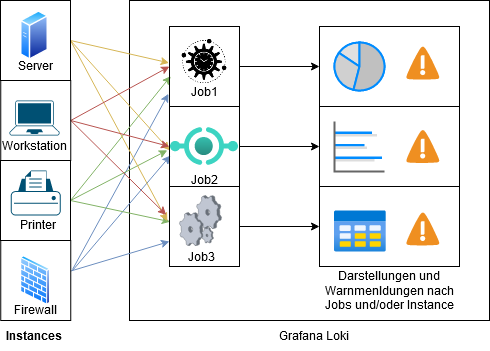
\includegraphics[width=0.8\textwidth]{assets/Instance_Jobs.drawio.png}
   \caption[Beziehung zwischen \quotes{instance} und \quotes{job}]
   {Beziehung zwischen \quotes{instance} und \quotes{job}}
   \label{fig:Labels_GrafanaLoki}
   \centering
\end{figure}

\newpage
Der Inhalt Logdateien kann dann in Grafana nach dem definierten Labels aufgerufen werden, wie auf der folgenden Abbildung \ref{fig:screenshot_labels} dargestellt:

\begin{figure}[H]
   \centering
   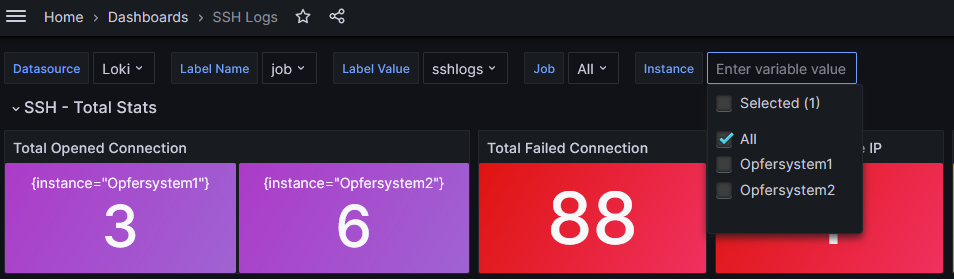
\includegraphics[width=0.7\textwidth]{assets/Grafana_labels.png}
   \caption[Aufrufe des Inhalts der Logdateien nach bestimmten Labels]
   {Aufrufe des Inhalts der Logdateien nach bestimmten Labels}
   \label{fig:screenshot_labels}
   \centering
\end{figure}

Mit \gls{logql} können auch Filterung verwendet, um nach bestimmten \quotes{instance} und/oder \quotes{jobs} die Daten aufzurufen, wie auf der Abbildung \ref{fig:screenshot_logql} dargestellt:

\begin{figure}[H]
   \centering
   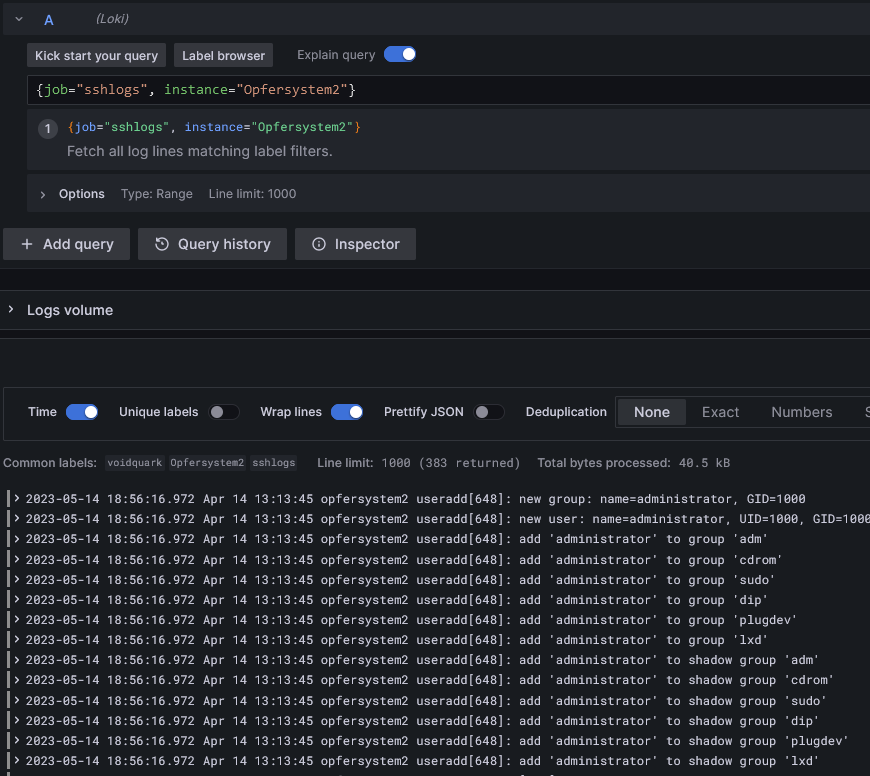
\includegraphics[width=0.7\textwidth]{assets/Logql_labels.png}
   \caption[Aufrufe des Inhalts der Logdateien mit \gls{logql}]
   {Aufrufe des Inhalts der Logdateien \gls{logql}}
   \label{fig:screenshot_logql}
   \centering
\end{figure}

In dem nächsten Abschnitt beschreiben wir, wie diese Regel in \gls{logql} geschrieben werden.

\newpage
\subsubsection{Regelsätze in LogQL}
In diesem Abschnitt fassen wir zusammen, wie eine Abfrage in \gls{logql} für eine Logdatei mit \gls{ssh} Einträgen aussieht. Für ausführliche Informationen über den Aufbau der Abfrage verweisen wir die offizielle Dokumentation, auf die diese Erklärung basiert ist \citep{Grafana_logql}. Unsere Logdatei enthält unter anderem folgende Zeile:

{\setstretch{1.0}
\begin{Verbatim}[frame=single]
14 14:05:30 opfersystem2 sshd[1698]: Failed password for administrator
from 10.0.2.15 port 58036 ssh2
\end{Verbatim}
}

Um fehlgeschlagene Anmeldeversuche zu erkennen, extrahieren wir folgende Felder aus den \gls{ssh}-Logdateien. Diese Information verwenden wir um gleiche Events zu erkennen und deren Anzhal festzustellen.

{\setstretch{1.0}
\begin{Verbatim}[commandchars=\\\{\},frame=single]
14 14:05:30 opfersystem2 \textbf{\textcolor{red}{sshd[}}1698]: \textbf{\textcolor{red}{Failed}} password for \textbf{\textcolor{blue}{administrator}}
from \textbf{\textcolor{blue}{10.0.2.15}} port 58036 ssh2
\end{Verbatim}
}

Wir teilen die Abfrage unten mit, um ihre Bestandteile besser zu verstehen:

\begin{table}[H]
   \setstretch{1.2}
   \begin{tabularx}{\textwidth}{|m{5cm}|X|}
   \hline
   \multicolumn{1}{|c|}{\textbf{\gls{logql}-Codeschnipsel}} & \multicolumn{1}{|c|}{\textbf{Beschreibung}} \\
   \hline
   \centering
   sum by(add)
   (rate(\{job=\verb|"|\textit{JOBNAME}\verb|"|
   instance=~\verb|"|\$instance\verb|"|\}

   & Hiermit wird die Aufsummierung der Benutzernamen definiert, die wir mit \quotes{Patterns} in \gls{logql} definiert haben. \quotes{Patterns} ermöglichen die einfache Extrahierung von Informationen aus einer Zeile. Wir holen alle Log-Einträge, die sich auf den von uns definierten Job beziehen. Wir können auch nach spezifischen Endpoint filtern, indem wir das Schlüsselwort \quotes{instance} benutzen. \\
   \hline
   \centering
   |
   & \quotes{|} funktioniert in \gls{logql} wie eine Pipeline für die Verkettung von mehreren Suchmustern. \\
   \hline
   \centering
         |= \lq \textbf{\textcolor{red}{sshd}}[\rq
      \\ |= \lq: \textbf{\textcolor{red}{Failed}}\rq
    &
    Suche nach Zeilen mit den in den rot markierten Einträgen. \\
   \hline
   \end{tabularx}
\end{table}

\begin{table}[H]
   \setstretch{1.2}
   \begin{tabularx}{\textwidth}{|m{5cm}|X|}
   \hline
   \multicolumn{1}{|c|}{\textbf{Element}} & \multicolumn{1}{|c|}{\textbf{Beschreibung}} \\
   \hline
   \centering
      !\verb|~| \lq \textbf{\textcolor{red}{invalid user}}\rq \\
      !\verb|~| \lq \textbf{\textcolor{red}{Legitimer\_Nutzer}}\rq \\
      !\verb|~| \lq \textbf{\textcolor{red}{Legitime\_Adresse}}\rq
   & Suche nach Zeilen \textbf{ohne} diese Einträge. Wir können beispielsweise Einträge ausschließen, die auf legitimen Nutzer oder IP-Adresse beziehen, um falsche Positive zu vermeiden \\
   \hline
   \centering
      | pattern \lq<\_> for \\
      <\textbf{\textcolor{blue}{Benutzername}}> from \\
      <\textbf{\textcolor{blue}{Quelladresse}}> port <\_>\rq \\
      \verb|[|\$ \verb|__|range\verb|]|\verb|))|

   & Die Definition der Wörter \quotes{Benutzername}, \quotes{Quelladresse} und als \quotes{Patterns} dienen dazu, einen Benutzernamen und eine Quelle IP-Adresse aus der Logdatei zu extrahieren. Die Platzhalter \quotes{<\_>} sind unbenannte Elemente, die in diesem Fall auf die Einträge \quotes{password} und \gls{port} in der Zeile verweisen. \\
   \hline
   \end{tabularx}
   \caption[Elementen eines Regelsätzes in Grafana Loki]
   {Elementen eines Regelsätzes in Grafana Loki \\Quelle: Eigene Quelle, \citep{VoidQuark_sshlogs} und \citep{Setter_Logfmt}}
\end{table}


% \begin{table}[H]
%    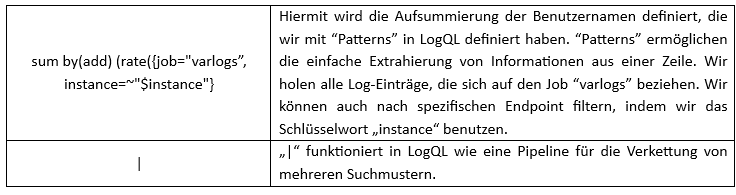
\includegraphics[width=1\linewidth]{assets/tabelle_logql_1.png}
% \end{table}

% \begin{table}[H]
%    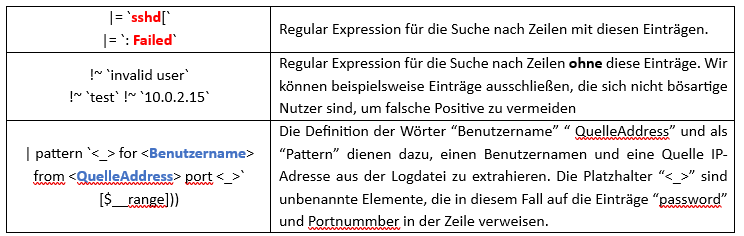
\includegraphics[width=1\linewidth]{assets/tabelle_logql_2.png}
%    \caption[Aufbau der Regelsätze in Grafana Loki für \gls{ssh} Logdateien]
%    {Aufbau der Regelsätze in Grafana Loki für \gls{ssh} Logdateien \\Quelle: Eigene Quelle, \citep{VoidQuark_sshlogs} und \citep{Grafana_logql}}
% \end{table}

Schließlich sieht der Regelsatz so aus:

{\setstretch{1.0}
\begin{Verbatim}[fontsize=\small, commandchars=\\\{\}, frame=single]
sum by(add) (rate({job="\textit{JOBNAME}", instance=~"$instance"} |= '\textbf{\textcolor{red}{sshd}}[' |= ':
\textbf{\textcolor{red}{Failed}}' !~ '\textbf{\textcolor{red}{invalid user}}' !~ '\textbf{\textcolor{red}{Legitimer_Nutzer}}' !~ '\textbf{\textcolor{red}{Legitime_Adresse}}' |
pattern '<_> for <\textbf{\textcolor{blue}{Benutzername}}> from  <\textbf{\textcolor{blue}{Quelladresse}}> port <_>' [$__range]))
\end{Verbatim}
}

% \begin{table}[H]
%    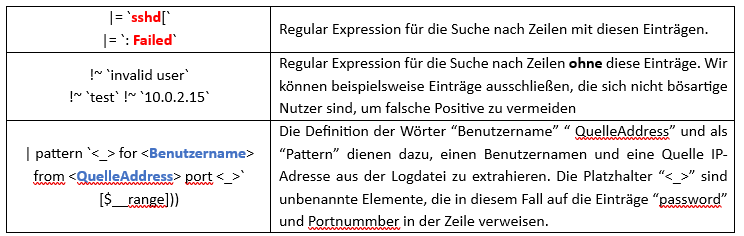
\includegraphics[width=1\linewidth]{assets/tabelle_logql_2.png}
%    \caption[Aufbau der Regelsätze in Grafana Loki für \gls{ssh} Logdateien]
%    {Aufbau der Regelsätze in Grafana Loki für \gls{ssh} Logdateien \\Quelle: Eigene Quelle, \citep{VoidQuark_sshlogs} und \citep{Grafana_logql}}
% \end{table}

Eine allgemeine Erkennungsregel in \gls{logql} würde so aussehen:
{\setstretch{1.0}
\begin{Verbatim}[frame=single]
Ergebnis = Operation (GesuchterWert) (Operation(label1="LabelWert",
label2="Label2Wert") |= 'Gesuchte Inhalt im Logdatei' | !'Inhalt im
Logdatei ausschliessen' | Regulärer Ausdrucke | pattern '<_>
WortImLogDatei <GesuchterInhalt> WortImLogDatei <_>' [\$__range]))
\end{Verbatim}
}

% {\setstretch{1.0}
% \begin{Verbatim}[fontsize=\small, commandchars=\\\{\}, frame=single]

% # Ergebnis wird mithilfe von \gls{logql} aus der Logdatei extrahiert.
% Ergebnis = Operation (GesuchterWert) (Operation(label1="LabelWert", label2="Label2Wert") |= 'Gesuchte Inhalt im Logdatei' | !'Inhalt im Logdatei ausschliessen' | Regulärer Ausdrucke | pattern '<_> WortImLogDatei <GesuchterInhalt> WortImLogDatei <_>' [$__range]))

% # FehlVersuche = Festgelegter Anzahl von fehlgeschlagenen Anmeldungsversuchen
% für das Triggern von Warnmeldung

% # \quotes{Operation} bezieht sich auf die Funktionen in Logql, z.B. für Aufsummierung,
% Mittelwert.

% \textit{while} Ergebnis < FehlVersuche
%    weiterBeobachten\(\)
% WarnmeldungTriggern\(\)

% \end{Verbatim}
% }

\newpage
\subsection{Hinzufügen der Regelsätze Grafana Loki}
Die Regelsätze in Grafana Loki können sowohl \textbf{manuell} im Menü \quotes{Code} als auch über die \textbf{\gls{GUI}} im Menü \quotes{Builder} geschrieben werden. Letzteres bietet eine benutzerfreundlichere Umgebung, um die Regeln zu schreiben. Die folgenden Abbildungen, \ref{fig:Loki_Code} und \ref{fig:Loki_Builder}, zeigen diese beiden Optionen:

\begin{figure}[H]
   \centering
   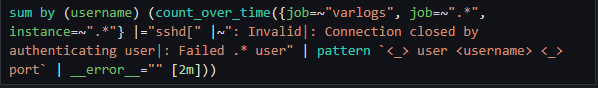
\includegraphics[width=0.85\textwidth]{assets/manuellerCodeLoki.png}
   \caption[Feld in Grafana Loki für die manuelle die Eingabe des \gls{logql}-Codes]
   {Feld in Grafana Loki für manuelle die Eingabe des \gls{logql}-Codes. \\ Quelle: \citep{VoidQuark_sshlogs}}
   \label{fig:Loki_Code}
   \centering
\end{figure}

\begin{figure}[H]
   \centering
   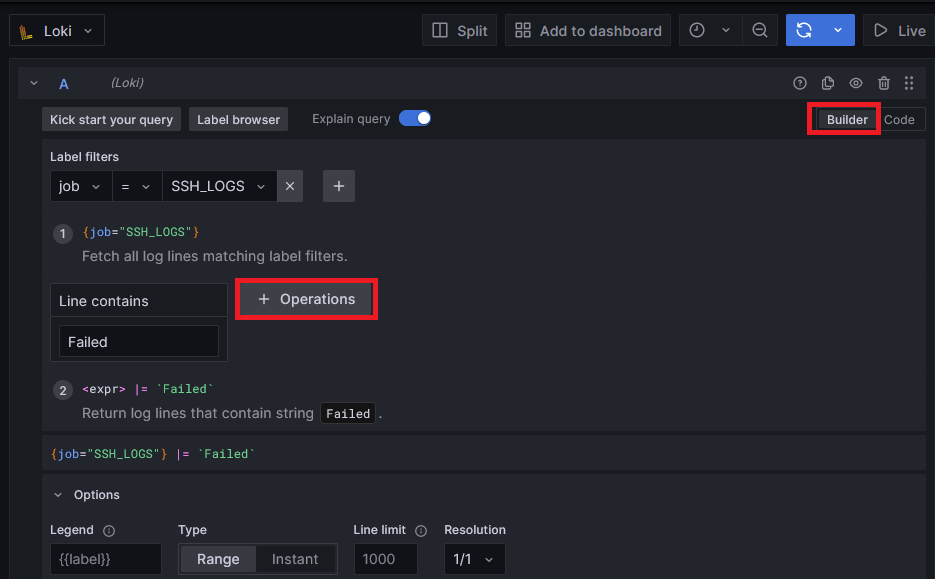
\includegraphics[width=0.85\textwidth]{assets/klickibuntyGrafana.png}
   \caption[\quotes{Builder} in Grafana Loki für nutzerfreundlichere Eingabe des \gls{logql}-Codes.]
   {\quotes{Builder} in Grafana Loki für nutzerfreundlichere Eingabe des \gls{logql}-Codes. Quelle: \citep{VoidQuark_sshlogs}}
   \label{fig:Loki_Builder}
   \centering
\end{figure}

\newpage
Beide Optionen bieten die Möglichkeit, eine Erklärung zur Abfrage anzuzeigen, wie auf der Abbildung \ref{fig:Loki_CodeInformation} gezeigt wird:
\begin{figure}[H]
   \centering
   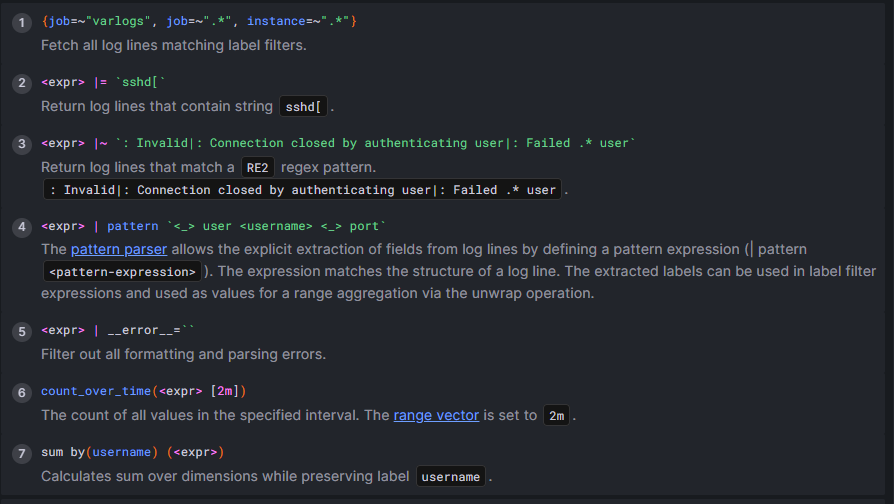
\includegraphics[width=1\textwidth]{assets/erklaerungLoki.png}
   \caption[Ausführliche Information über die Abfrage]
   {Ausführliche Information über die Abfrage\\Quelle: \citep{Grafana_QueryEditor}}
   \label{fig:Loki_CodeInformation}
   \centering
\end{figure}

Mit der Nutzung von \textit{\gls{API}} \gls{Endpoint} von Loki ist es möglich nach dem Inhalt der Logdateien abzufragen, indem die Regelsätze in \gls{logql} geschrieben werden. In diesem Fall bekommen wir die gefilterte Ergebnis als Antwort \citep{Grafana_api}.

{\setstretch{1.0}
\begin{Verbatim}[fontsize=\small, frame=single]
# Muster für die Anfrage
curl -G -s  "http://LokiInstance/Endpoint" --data-urlencode 'Logql Abfrage'
| jq

# Beispiel
curl -G -s  "http://LokiInstance/loki/api/v1/query" --data-urlencode
'sum by(add) (rate({job="JOBNAME", instance=~"$instance"} |= 'sshd[' |= ':
Failed' !~ 'invalid user' !~ 'Legitimer_Nutzer' !~ 'Legitime_Adresse' |
pattern '<_> for <Benutzername> from  <Quelladresse> port <_>' [$__range]))'
| jq
\end{Verbatim}
}

\newpage
\newgeometry{right=30mm, left=30mm}
\thispagestyle{lscape}
\begin{landscape}
   Nachdem die \gls{ssh}-Logdateien gelesen und verarbeitet wurden, bekommen wir von Grafana Loki die zusammenfassende Ergebnissen, wie unter auf der Abbildung \ref{fig:Grafana_DetailedStats} dargestellt:
    \begin{figure}[H]
       % \centering
        \centerline{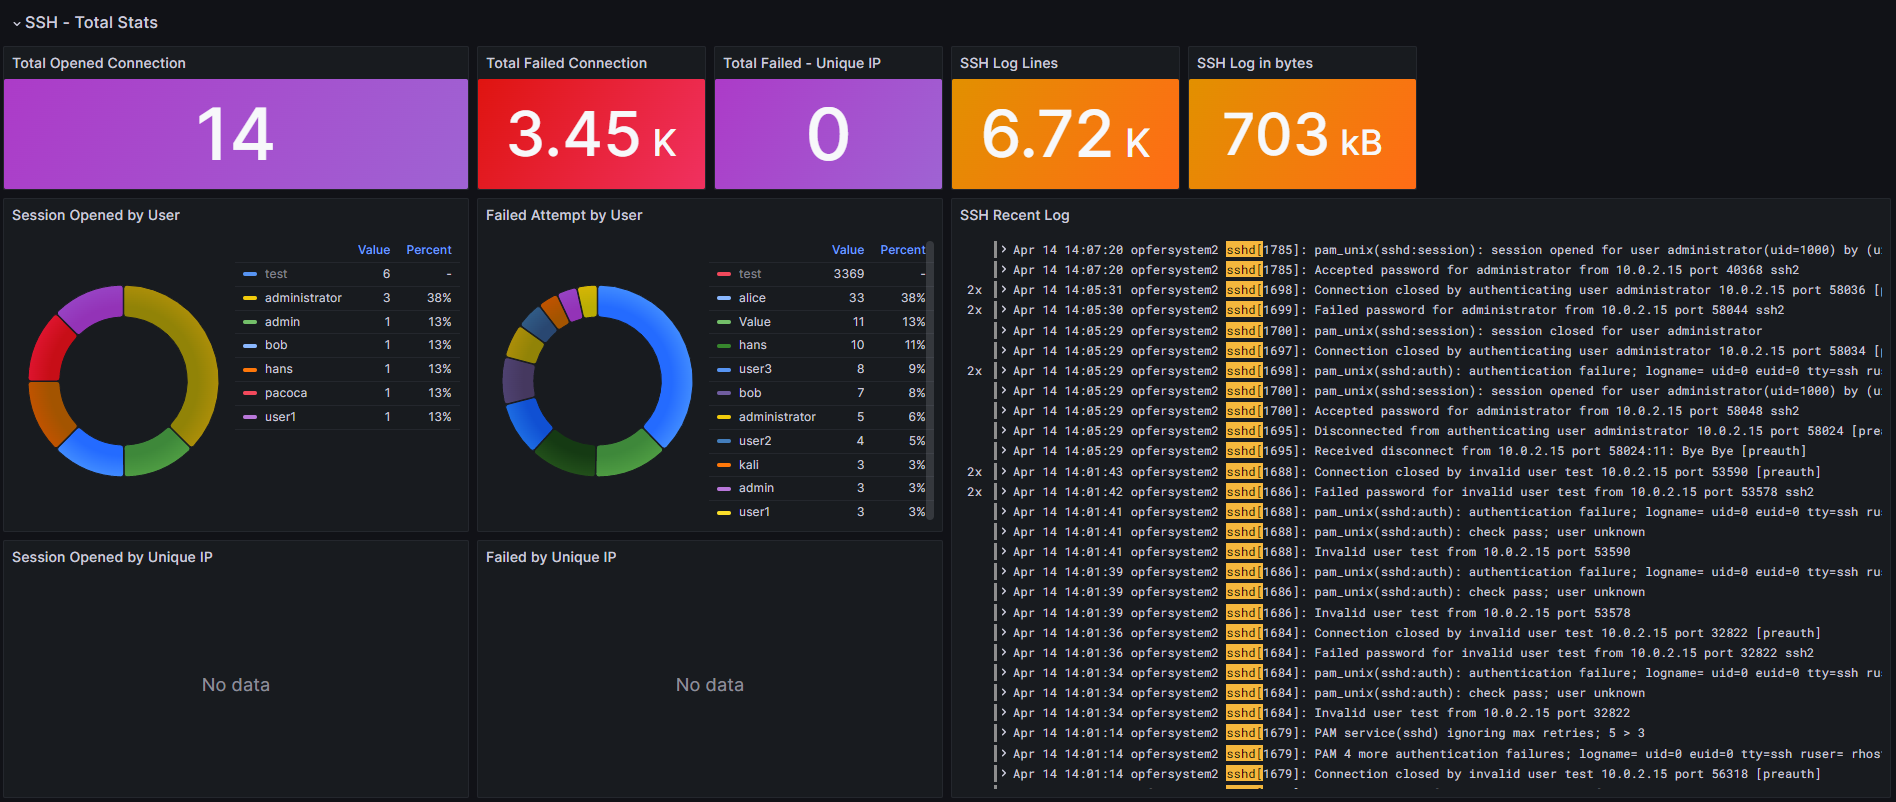
\includegraphics[width=1.7\textwidth]{assets/GrafanaLoki_ssh}}
        %\includegraphics[width=1.2\textwidth]{assets/5.4.2_1_Abb.jpeg}
        \caption[Ausgabe der Verarbeitung der \gls{ssh} Logdateien von Grafana Loki]
        {Ausgabe der Verarbeitung der \gls{ssh} Logdateien von Grafana Loki}
        \label{fig:Grafana_Grafik}
        \centering
    \end{figure}
\end{landscape}
\restoregeometry

\newpage
\newgeometry{right=30mm, left=30mm}
\thispagestyle{lscape}
\begin{landscape}
   Das nächste Abbidung, \ref{fig:Grafana_DetailedStats}, gibt ausführliche Informationen der Logdateien:
    \begin{figure}[H]
       % \centering
        \centerline{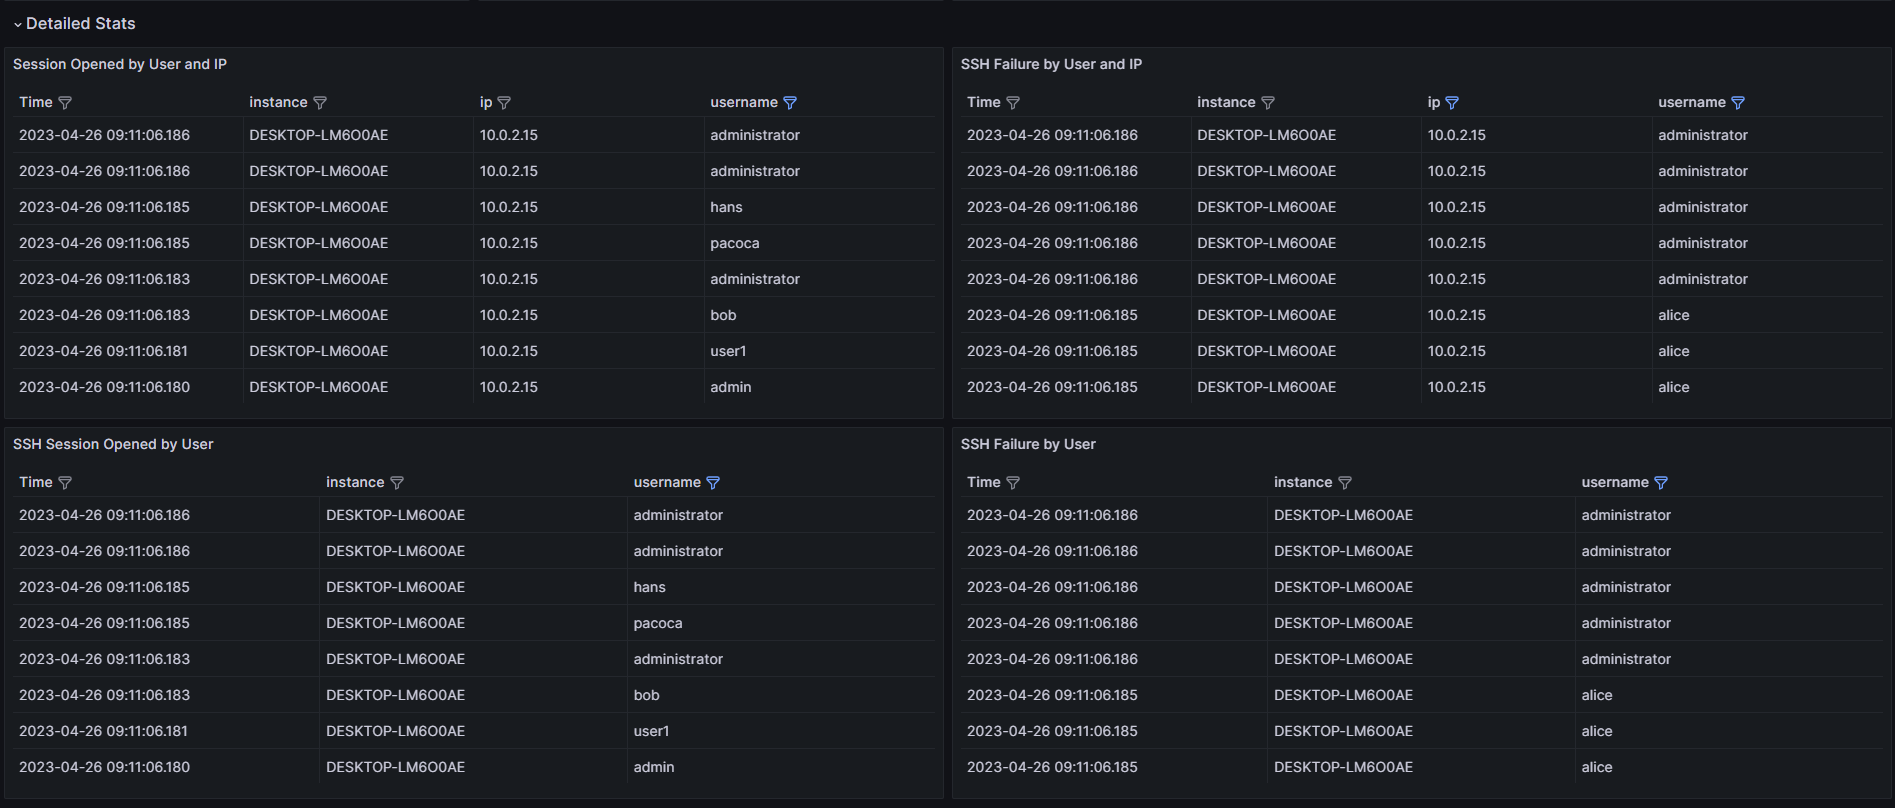
\includegraphics[width=1.7\textwidth]{assets/GrafanaLoki_sshDetailed.png}}
        \caption[Ausführliche Darstellung der \gls{ssh} Logdateien von Grafana Loki]
        {Ausführliche Darstellung der \gls{ssh} Logdateien von Grafana Loki}
        \label{fig:Grafana_DetailedStats}
        \centering
    \end{figure}
\end{landscape}
\restoregeometry

% \thispagestyle{lscape}
% \begin{landscape}
%    Das nächste Bild gibt ausführliche Informationen der Logdateien:
%    \begin{center}
%       \begin{figure}[H]
%          \centering
%          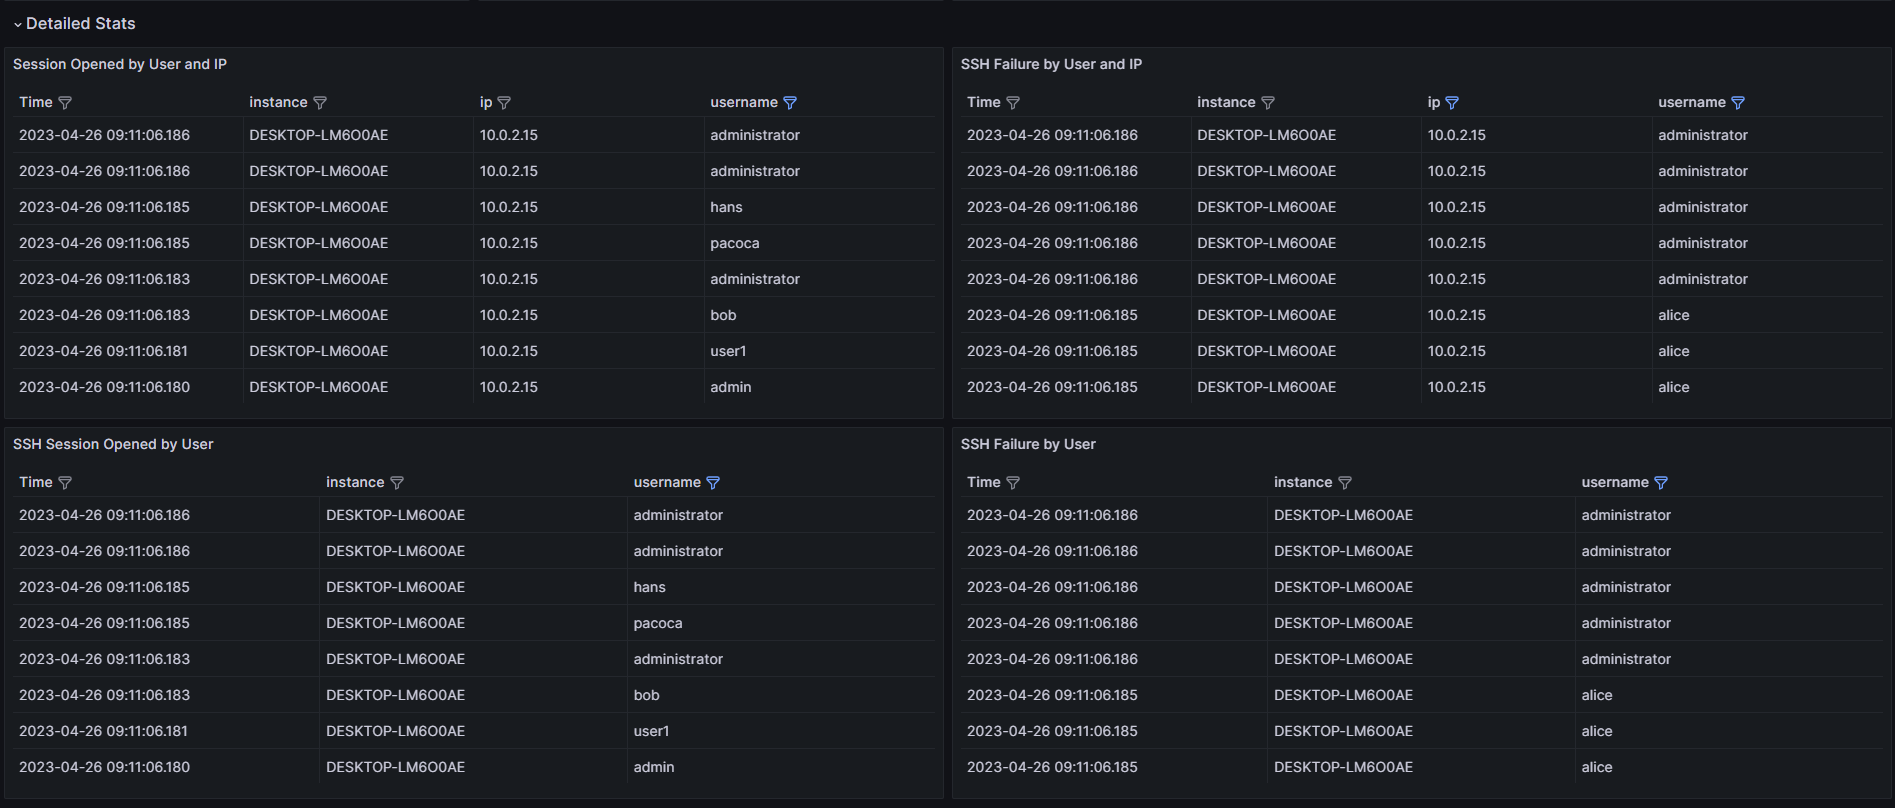
\includegraphics[width=1.3\textwidth]{assets/GrafanaLoki_sshDetailed.png}.
%          \caption[Ausführliche Darstellung der \gls{ssh} Logdateien von Grafana Loki]
%          {Ausführliche Darstellung der \gls{ssh} Logdateien von Grafana Loki\\Quelle: Eigene Quelle and \citep{VoidQuark_sshlogs}}
%          \centering
%       \end{figure}
%    \end{center}
% \end{landscape}

\subsection{Einrichtung der Warnmeldungen in Grafana}
In den vorherigen Teilen dieser Arbeit haben wir uns damit auseinandergesetzt, Grafana so einzurichten, dass wir schließlich eine Lösung ähnlich einer \gls{SIEM} erhalten. Von unseren ursprünglichen Ziele haben wir bereits Folgendes erreicht:

{\setstretch{1}
\begin{enumerate}[noitemsep]
   \item	Sammlung der Logdateien von den \glsplural{Endpoint} mit Promtail
   \item Anpassung der Logdateien für die Weiterleitung an Grafana Loki
   \item Nutzung von Regelsätzen in Loki für die Analysierung der \gls{ssh} Logdateien
   \item Graphische Darstellung der Ergebnissen in Grafana mit den in Loki verwendeten Regelsätzen
\end{enumerate}
}

Unser letztes Ziel besteht darin, Warnmeldungen für potenzielle Angriffe mithilfe der Ergebnisse von Loki zu generieren. Grafana kann sowohl intern mit der Funktionalität \quotes{Alerting} als auch extern mit \glsplural{plugin}, wie \textbf{Alertmanager}, Warnmeldungen generieren. Der zweite kann Daten von \gls{prometheus}, \gls{cortex} und \gls{mimir} als Datenquelle verwenden \citep{Grafana_Alertmanager} und kann Daten von beliebigen \glsplural{Endpoint} empfangen. Die Regelsätze des Alertmanagers haben folgendes Muster:

{\setstretch{1.0}
\begin{Verbatim}[frame=single]
# Warnmeldungen können in beliebigen Gruppen kategorisiert werden. Diese
können von den Nutzern entsprechend ihrer Anforderungen und Bedürfnisse
definiert werden.
groups:
      # Ab diesem Punkt beginnen wir mit der Definition der Regelsätze
      für die Erkennung von Warnmeldungen. Diese umfassen:
   - name: example
     rules:
    - alert: HighRequestLatency

      # LogQL-Regelsätze für die Erkennung der Warnmeldung, welche die
      in den vorherigen Schritten definierten Abfragen verwenden.
      expr: job:request_latency_seconds:mean5m{job="SSH_LOGS"} > 0.5
      for: 10m
       labels:
         severity: page
       annotations:
         summary: High request latency
\end{Verbatim}
}

%verbatim comments
%lst listing
\newpage
Grafana hat auch ein eigenes internes Tool, um Warnmeldungen zu konfigurieren: \textbf{Alerting}. In dieser Arbeit versuchen wir unser Warnmeldungs-System mithilfe dieses Tools aufzubauen.

Die Warnmeldungen können direkt in der \gls{GUI} von Grafana konfiguriert werden. Dazu folgt man den folgenden Schritten \citep{Grafana_alerting}:

{\setstretch{1}
\begin{enumerate}[noitemsep]
   \item Name der Regel
   \item Regelsätze in \gls{logql}
   \item Definition von Gruppen für jede Art von Warnmeldung. Gruppen können später verschiedenen Einstellungen zugewiesen werden, wie z.B. Benachrichtigungen und Inhalte.
   \item Informationen über die Warnmeldung, wie eine eindeutige ID und eine Beschreibung. Der Nutzer kann diese Felder so definieren, wie es notwendig ist.
   \item Benachrichtigung der Zielgruppe, die diesen Fall später bearbeiten wird.
   \item Labels zur besseren Organisation der Warnmeldungen.
   \item Konfiguration von E-Mail in Grafana für die Weiterleitung der Warnmeldungen.
\end{enumerate}
}

Für unseren ersten Test erstellen wir Warnmeldungen über die \textbf{\gls{GUI}} von Grafana für fehlgeschlagene Anmeldeversuche. Wir haben die oben genannten Elemente definiert und die folgenden Regelsätze verwendet \citep{VoidQuark_sshlogs}:

{\setstretch{1.0}
\begin{Verbatim}[frame=single]
# (A) Anzahl von fehlgeschlagenen Anmeldeversuche für existierenden
Benutzernamen:
sum by (username) (count_over_time({$label_name=~"$label_value",
job=~"$job", instance=~"$instance"} |="sshd[" |~": Invalid|:
Connection closed by authenticating user|: Failed .* user" |
pattern '<_> user <username> <_> port' | __error__=""
[$__interval]))

# (B) Anzahl von Fehlgeschlagenen Anmeldeversuche für nicht
existierenden Benutzernamen:
sum by (username) (count_over_time({$label_name=~"$label_value",
job=~"$job", instance=~"$instance"} |="sshd[" |=": Failed" !~"invalid
user" | pattern '<_> for <username> from <_> port' | __error__=""
[$__interval]))

# Wenn die Anzahl von (A) oder von (B) größer als fünf ist, dann wird
die Warnmeldung als E-Mail an dem Ziel geschickt.
\end{Verbatim}
}

% discard lines with Server Ansible - https://grafana.com/docs/loki/latest/logql/log_queries/

Im Anhang \ref{appendix:Warnmedungskonfiguration} befindet sich die Konfigurationsdatei für unsere Warnmeldung.

Nachdem alles korrekt konfiguriert wurde, haben wir die folgende E-Mail erhalten:
\begin{figure}[H]
   \centering
   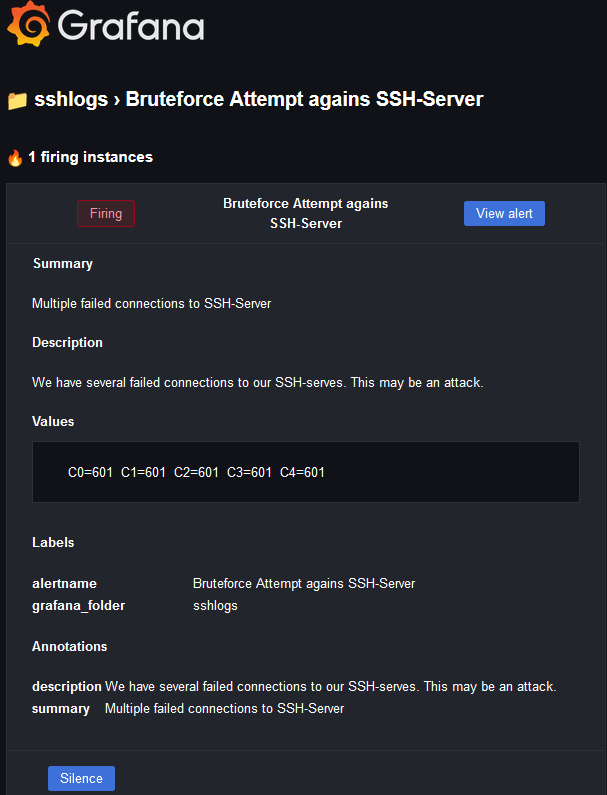
\includegraphics[width=0.7\textwidth]{assets/GrafanaWarnmeldung.png}
   \caption[E-Mail Warnmeldung von Grafana]
   {E-Mail Warnmeldung von Grafana}
   \centering
\end{figure}

%Grafana ermöglichte älterer Versionen (bevor v0.9) Warnmeldungen über die \gls{API} zu generieren \citep{Grafana_AlertLegacyApi}.

%Das Alerting-Tool von Grafana bietet keine direkte Integration zu einem \gls{IDS}, \gls{IPS}, \gls{SIEM} oder einer \gls{API} an. Die Kommunikation mit solchen \glsplural{Endpoint} lässt sich jedoch mithilfe von \textbf{\gls{webhook}} konfigurieren \citep{Grafana_Notifications}.

% enabled = true
% host = smtp.gmail.com:587
% user = alertsgrafanaBA@gmail.com
% # If the password contains # or ; you have to wrap it with triple quotes. Ex """#password;"""
% password = "sexpjkbdsdwrkgqm"
%skip_verify = true

%Password: alertsgrafanaBA1


